\documentclass{article}



\usepackage{arxiv}

\usepackage[utf8]{inputenc} % allow utf-8 input
\usepackage[T1]{fontenc}    % use 8-bit T1 fonts
\usepackage{hyperref}       % hyperlinks
\usepackage{url}            % simple URL typesetting
\usepackage{booktabs}       % professional-quality tables
\usepackage{amsfonts}       % blackboard math symbols
\usepackage{nicefrac}       % compact symbols for 1/2, etc.
\usepackage{microtype}      % microtypography
\usepackage{lipsum}		% Can be removed after putting your text content
\bibliographystyle{abbrv}
\usepackage{graphicx}
\usepackage{subcaption}
\usepackage{natbib}
\usepackage{doi}
\usepackage{float}

\usepackage{bm}% http://ctan.org/pkg/bm

\usepackage{amsmath}
\usepackage{amssymb}
\DeclareMathOperator*{\argmin}{arg\,min}

\usepackage{hyperref}
\usepackage{cleveref}
\usepackage[toc,page]{appendix}

\title{Probabilistic Machine Learning – Exam}

%\date{September 9, 1985}	% Here you can change the date presented in the paper title
%\date{} 					% Or removing it

\author{Jeppe Søndergaard Johansen (PVC439), Jonas Raaschou-Pedersen (FJR906), Julius Løve Fischer (NBM205)}

% Uncomment to remove the date
%\date{}

% Uncomment to override  the `A preprint' in the header
%\renewcommand{\headeright}{Technical Report}
%\renewcommand{\undertitle}{Technical Report}
%\renewcommand{\shorttitle}{\textit{arXiv} Template}

%%% Add PDF metadata to help others organize their library
%%% Once the PDF is generated, you can check the metadata with
%%% $ pdfinfo template.pdf

%\hypersetup{
% pdftitle={Probabilistic Machine Learning – Exam},
% pdfsubject={q-bio.NC, q-bio.QM},
% pdfauthor={Jeppe Søndergaard Johansen, Jonas Raaschou-Pedersen, Julius Løve % Fischer},
%pdfkeywords={First keyword, Second keyword, More},}

\begin{document}
\maketitle

%\begin{abstract}
%	\lipsum[1]
%\end{abstract}

% keywords can be removed
% \keywords{First keyword \and Second keyword \and More}

\section*{A – Density modeling\footnote{The associated code for the report is available at the following \href{https://github.com/jsr-p/pmldiku-exam-paper}{Github repository.}}}

\subsection*{A.1 – Implement a convolutional VAE}
The setup of the variational autoencoder model is the assumption of 
a deep latent variable model (DLVM), which is a latent variable model 
$p_{\bm{\theta}}(\mathbf{x}, \mathbf{z})$ whose distributions are parameterized
by a deep neural network \citep{Kingma_2019}. 
We are interested in conducting inference on the posterior distribution 
$p_{\bm{\theta}}(\mathbf{z} \mid  \mathbf{x})$, which
by Bayes' rule can be written as
    \begin{align}
        \label{posterior_dlvm}
        p_{\bm{\theta}}(\mathbf{z} \mid  \mathbf{x})
        = 
    \frac{p_{\bm{\theta}}(\mathbf{x}, \mathbf{z})}{p_{\bm{\theta}}(\mathbf{x})}.
    \end{align}
For DLVMs the marginal likelihood $p_{\bm{\theta}}(\mathbf{x})$ and the posterior $p_{\bm{\theta}}(\mathbf{z} \mid  \mathbf{x})$ are intractable.
However, approximate inference is possible using the variational autoencoder. The variational autoencoder posits a parametric inference model
$q_{\phi}(\mathbf{z} \mid \mathbf{x})$ called the encoder. The vector
$\mathbf{\phi}$ consists of the variational parameters which are optimized such
that the encoder approximates the posterior distribution as shown in equation
\eqref{posterior_dlvm}. The main objective is the evidence lower bound (ELBO):  
\begin{align}
    \label{ELBO}
    \mathcal{L}_{\bm{\theta}, \bm{\phi}}(\mathbf{x})
    &= \mathbb{E}_{q_{\bm{\phi}}(\mathbf{z} \mid  \mathbf{x})} \left[
        \log p_{\bm{\theta}}(\mathbf{x}, \mathbf{z})
        - \log q_{\phi}(\mathbf{z} \mid \mathbf{x})
    \right] \\
    &= 
    - \mathrm{KL} \left( q_{\phi}(\mathbf{z} \mid \mathbf{x}) \mid  p_{\bm{\theta}}(\mathbf{z}) \right) 
    + 
    \mathbb{E}_{q_{\bm{\phi}}(\mathbf{z} \mid  \mathbf{x})} \left[
        \log p_{\bm{\theta}}(\mathbf{x} \mid  \mathbf{z})
    \right].
\end{align}

To optimize the objective in \eqref{ELBO} with respect to $\bm{\phi}$ and $\bm{\theta}$
we use the reparametrization trick \cite{Kingma_2019}.
This allows us to estimate the individual-datapoint ELBO \eqref{ELBO} 
using a simple Monte Carlo estimator:
first we sample a noise term $\bm{\epsilon} \sim p(\bm{\epsilon}) = \mathcal{N}(\bm{\epsilon}; \bm{0}, \bm{I})$ from a multivariate standard normal distribution; then we pass it through a function 
$\mathbf{z} = g(\bm{\phi}, \bm{\theta}, \bm{\epsilon})$ and finally we evaluate 
\begin{align}
    \label{sp-ELBO}
    \tilde{\mathcal{L}}_{\bm{\theta}, \bm{\phi}}(\mathbf{x}) 
    =
    q_{\bm{\phi}}(\mathbf{z} \mid  \mathbf{x}) -
    \log p_{\bm{\theta}}(\mathbf{x} \mid  \mathbf{z}).
\end{align}
Using the reparametrization trick the gradient $
    \nabla_{\bm{\theta}, \bm{\phi}}\tilde{\mathcal{L}}_{\bm{\theta}, \bm{\phi}}(\mathbf{x}) 
$
is readily optimized using the autodifferentiation framework of PyTorch \cite{pytorch}.

\subsubsection*{Factorized Gaussian Encoder}
In all of our models we assume that the encoder 
is a Gaussian encoder with diagonal covariance matrix 
\begin{align}
    q_{\phi}(\mathbf{z} \mid \mathbf{x}) 
    &= \mathcal{N}(\mathbf{z}; \bm{\mu}, \bm{\sigma}^2 \mathbf{I}) \\ 
    (\bm{\mu}, \log \bm{\sigma}^2) 
    &= \mathrm{EncoderNeuralNet}_{\bm{\phi}}(\mathbf{x}).
\end{align}

The resulting estimator for a single datapoint equals 
\begin{align}\label{eq7}
    \tilde{\mathcal{L}}_{\bm{\theta}, \bm{\phi}}(\mathbf{x}) 
    &=
    \frac{1}{2} \sum_{j=1}^{J} \left( 
    1 + \log \sigma^2_j - \mu_{j} - \sigma^2_{j}
    \right) 
    + \log p_{\bm{\theta}}(\mathbf{x} \mid  \mathbf{z}) \\ 
    \text{where  }  \mathbf{z} &= \bm{\mu} + \bm{\sigma} \odot \bm{\epsilon}, \ \
    \bm{\epsilon} \sim  \mathcal{N}(\bm{0}, \bm{I}).
\end{align}

\subsubsection*{Decoder}
The term  $\log p_{\bm{\theta}}(\mathbf{x} \mid  \mathbf{z})$ takes three different forms depending on our three separate assumptions – that $p_{\bm{\theta}}(\mathbf{x} \mid  \mathbf{z})$ is (1) Gaussian  distributed, (2) Bernoulli distributed or (3) Continuous Bernoulli  distributed. Assumption (1) is motivated by the fact that the standardized MNIST data is continuous in the $[0,1]$-interval. However in practice, the distribution of the pixels in MNIST are largely centered on 0 and 1 favoring the Bernoulli assumption. These two considerations jointly motivate the third assumption: the assumption of the pixels following a continuous Bernoulli (CB) distribution \cite{CB}. This is a novel distribution specifically created because of the considerations of the pixels neither being normal or Bernoulli distributed. Instead, the CB distribution models a continuous variable in $[0, 1]$-interval; exactly as the digits in the normalized MNIST data.  
Considering the loss function used in estimating the VAE, under assumption 1. we use the mean-squared error (MSE) for the reconstruction error in \eqref{eq7}, whereas 2. implies binary cross-entropy loss (BCE), and 3. implies BCE plus the normalizing constant of the continuous Bernoulli distribution (see \cite{CB}). 
For all of the three assumptions we model the decoder as a parametrized neural net.



\subsection*{A.2 – Alternative models}
\subsubsection*{Fully Bayesian VAE}
As written in \citep{BVAE}, a full Bayesian analysis of the VAE is possible. This analysis allows us to perform variational inference on
the latent variables $\mathbf{z}$ and the parameters of $\bm{\theta}$.

We assume a hyperprior on the decoder's parameters; we assume the hyperprior has a multivariate standard normal density $p_{\bm{\alpha}}(\bm{\theta})$. 
The approximate posterior of $\bm{\theta}$ is denoted by $q_{\bm{\phi}}(\bm{\theta})$. 
In order to perform variational inference and make 
$q_{\bm{\phi}}(\bm{\theta})$ a good approximation to 
 $p_{\bm{\alpha}}(\bm{\theta} \mid \mathbf{X})$ we have to backpropagate through the parameters of the approximate posterior $q_{\bm{\phi}}(\bm{\theta})$. 
 To make this operational we apply the reparametrization trick a second time. 
The loss for a single datapoint is now given by 
\begin{align}
    \label{elbobayes}
	\tilde{\mathcal{L}}_{\bm{\theta}, \bm{\phi}}(\mathbf{x})
    &= 
	\log p_{\bm{\theta}}(\mathbf{x} \mid  \mathbf{z})
    + 
	\log p_{\bm{\theta}}(\mathbf{x})
    - 
	q_{\bm{\phi}}(\mathbf{z} \mid  \mathbf{x})
    + 
	\log p_{\bm{\alpha}}(\mathbf{x})
    - 
	\log q_{\bm{\phi}}(\mathbf{z}), \\ 
    \nonumber
	\text{where  }  
    \mathbf{z} & = \bm{\mu} + \bm{\sigma} \odot \bm{\epsilon}, \ \
    \bm{\theta} = \bm{\mu}_{\bm{\theta}} 
    + \bm{\sigma}_{\bm{\theta}} \odot \bm{\zeta} , \ \
	\bm{\epsilon}, \ \bm{\zeta}  \sim  \mathcal{N}(\bm{0}, \bm{I}).
\end{align}
The loss function is identical to the one in \eqref{eq7} 
with the the term
$\log q_{\bm{\phi}}(\mathbf{z})$
added. The same assumptions as before apply to the term $\log p_{\bm{\theta}}(\mathbf{x} \mid \mathbf{z})$.

\subsubsection*{Denoising Diffusion Probabilistic Models}
We implement a diffusion model as a SOTA generative image model \cite{diffusion2020}. We briefly give a summary of the model. Fundamentally, the model's encoding part consists of additively adding Gaussian noise to images. This goes on for $T$ steps until the original image is indistinguishable from Gaussian noise. More precisely we can consider the noise process a Markov chain of the form as described in \cite[p. 860, eq. 25.1]{pml2Book}:

\begin{equation}
    q(x_t \mid x_{t-1}) = \mathcal{N}(x_t \mid \sqrt{1 - \beta_t} x_{t-1}, \beta_t\mathbf{I})
\end{equation}

$\beta_t \in (0, 1)$ is chosen to follow a schedule, which defines the amount of noise. Transforming these $\beta_t$'s yields $\alpha_t = 1 - \beta_t$ and from here we define $ \Pi_{s=1}^t \alpha_s$. Using this we can construct our loss function:

\begin{equation}
    \lambda_t\Vert \epsilon - \epsilon_\theta (\sqrt{\bar{\alpha}} x_0 + \sqrt{1-\bar{\alpha}}\epsilon, t) \Vert^2
\end{equation}

As described in \cite[p.863, eq. 25.23 and 25.24]{pml2Book} the model performs best when $\lambda_t$ is set to 1. In essence, we can consider the prediction problem as removing noise from a noisy image i.e. going from $x_t$ to $x_{t-1}$. From here we can consider the denoising problem as starting by sampling an "image" of multivariate Gaussian noise, and iteratively using the trained neural network. More formally, we can consider the de-noising problem as $p_{\theta}(x_{t-1}\mid x_t) = \mathcal{N}\left(x_{t-1} ; \mu_{\theta}(x_t, t), \Sigma_{\theta}(x_t, t)\right)$, where $\mu_\theta$ and $\Sigma_\theta$ denotes the neural parametrization of a neural network. We use a convolutional neural network to de-noise the images, where we embed the time-step dimension using sinusoidal transformation because neural networks struggle to embed time.
We sample  $t\sim \mathcal{U}(0, T), \epsilon \sim \mathcal{N}(0, 1)$ and we choose the $T=1000, \beta_{min} = 10^{-4}, \beta_{max} = 0.2$ as done in the original paper \cite{diffusion2020}, and we also generate the $\beta$'s with equal distance. We use both a standard convolutional net, and a U-Net architecture for the decoding neural network. We use the empirical mean and standard deviation for scaling inputs\footnote{Scaling the inputs turns out to be incredibly important. Originally we scaled by the pixels so min = -1 and max = 1, but we found the performance increased using the empirical mean and standard deviation of the data. The original paper uses a more intricate scaling procedure \cite{diffusion2020}, which probably could improve performance more had we had more time.}. 

\subsection*{Assessing Generative Models}

We consider three ways of assessing our general models: Visual inspection, marginal likelihood in the case of VAE-type models, and as a last measure we use the Fréchet inception distance (FID). 

\textbf{Visual Inspection:} In general, we find that the VAEs outperform the diffusion models. In particular, the simple convolutional implementation of a diffusion model seems to be totally unable to generate images. The U-Net implementation does fairly well at generating realistic digits, and one could argue that the quality of the digits are seemingly higher than the quality of digits that some of the VAEs can produce. For the baseline VAE, we find that the continuous Bernoulli assumption increases the quality of the generated images significantly. This also appears to be the best performing model for generating digits. The lower quality of the convolutional VAE may stem from the fact that we have considered an oversimplified convolutional network. 
Lastly, the Bayesian VAE is hit or miss with regards to the quality of generated images. This suggests that this model manages to model the latent space well for some regions but not for others, implying that the KL-part of the loss function not regularizing the embedding enough to a standard normal distribution. A way to address this could be to choose a prior that has more weight on the KL term, akin to what is done \cite{Higgins2016betaVAELB}. Further, the complex nature of a fully Baeysian VAE, and the many variational parameters to estimate, may also be the reason that it is difficult to train and get reasonable generative results.

\textbf{Marginal Likelihood:} The marginal (log) likelihood as a tool for model selection can be motivated by considering a posterior distribution over models, $p(m|X)$, in which we assume a uniform prior over models. Computing the MAP estimate of $p(m|X)$ is then equivalent to selecting the model with the highest marginal likelihood, $p(X|m)$. To estimate the marginal log-likelihood of the VAE models we use importance sampling as suggested in \cite{importancesampling}. The marginal log-likelihood can be rewritten as

\begin{align}
	\nonumber
	\log p_{\bm{\theta}}(\mathbf{x}) = \log \int p_{\bm{\theta}}(\mathbf{x}, \mathbf{z})
	\frac{q_{\phi}(\mathbf{z} \mid \mathbf{x})}{q_{\phi}(\mathbf{z} \mid \mathbf{x})}
	d \mathbf{z}                                                                                      
	                                 & =
	\nonumber
	\log \mathbb{E}_{q_{\bm{\phi}}(\mathbf{z} \mid  \mathbf{x})} \left[
		\frac{
			p_{\bm{\theta}}(\mathbf{x}, \mathbf{z})
		}{q_{\phi}(\mathbf{z} \mid \mathbf{x})}
	\right]                                                                                             \\
	\label{IS-VAE}
	\Leftrightarrow
	\log p_{\bm{\theta}}(\mathbf{x}) & \approx
	\log \frac{1}{L} \sum_{l=1}^{L}
	\frac{
		p_{\bm{\theta}}(\mathbf{x} \mid  \mathbf{z}^{(l)}) p_{\bm{\theta}}(\mathbf{z})
	}{
		q_{\phi}(\mathbf{z}^{(l)} \mid \mathbf{x})
	}
\end{align}

\iffalse

\begin{align}
	\nonumber
	\log p_{\bm{\theta}}(\mathbf{x}) & = \log \int p_{\bm{\theta}}(\mathbf{x}, \mathbf{z})
	\frac{q_{\phi}(\mathbf{z} \mid \mathbf{x})}{q_{\phi}(\mathbf{z} \mid \mathbf{x})}
	d \mathbf{z}                                                                                        \\
	                                 & =
	\nonumber
	\log \mathbb{E}_{q_{\bm{\phi}}(\mathbf{z} \mid  \mathbf{x})} \left[
		\frac{
			p_{\bm{\theta}}(\mathbf{x}, \mathbf{z})
		}{q_{\phi}(\mathbf{z} \mid \mathbf{x})}
	\right]                                                                                             \\
	\label{IS-VAE}
	\Leftrightarrow
	\log p_{\bm{\theta}}(\mathbf{x}) & \approx
	\log \frac{1}{L} \sum_{l=1}^{L}
	\frac{
		p_{\bm{\theta}}(\mathbf{x} \mid  \mathbf{z}^{(l)}) p_{\bm{\theta}}(\mathbf{z})
	}{
		q_{\phi}(\mathbf{z}^{(l)} \mid \mathbf{x})
	}
\end{align}

\fi

where $\mathbf{z}^{(l)} \sim q_{\phi}(\mathbf{z} \mid \mathbf{x}) $. 
Therefore, to estimate the marginal log likelihood for a single datapoint $\mathbf{x}$
we draw $L$ observations from the encoder and compute the expression in \eqref{IS-VAE}.
To get the estimate on the total test data we compute the expression in \eqref{IS-VAE} 
for each data point and take the average. 
To avoid numerical instability we use the log-sum-exp trick. Looking to table \ref{tab:loglik} we find that the bayesian model performers worst within each group of error distribution specification\footnote{\textit{MSE} denotes mean squared error, \textit{cb} denotes continuous Bernoulli, \textit{BCE} denotes binary cross-entropy}.

\begin{table}[ht]
    \centering
    \resizebox{\textwidth}{!}{\begin{tabular}{llllllllll}
    \toprule
    model       &  vanilla mse &  conv mse &  bayes mse &  vanilla bce &  conv bce &  bayes bce &  vanilla cb &  conv cb &  bayes cb \\
    \midrule
    $\log p(x)$ &       -11.63 &    -11.79 &     -31.97 &       -41.53 &    -42.51 &     -61.81 &     2033.23 &  2063.43 &   1988.12 \\
    \bottomrule
    \end{tabular}}
    \caption{Marginal log likelihood}
    \label{tab:loglik}
\end{table}
\textbf{Fréchet Inception Distance:} The FID is found by measuring the distance in the embedding space of a classifier between real data and generated data. More concretely we train a convolutional neural network on the MNIST data\footnote{It predicts the correct label with a $97\%$ probability.}, and use the last embedding layer before the prediction to calculate the distance between the real (denoted $R$) and generated (denoted $G$) assuming both follow normal distributions. 

\begin{equation}
    FID = \Vert \mu_R - \mu_G \Vert_2^2 + \mathrm{tr}(\Sigma_R + \Sigma_G - 2 (\Sigma_R \Sigma_G)^{1/2})
\end{equation}

Note that lower distance implies a higher quality of generated images. Following \cite[p. 775]{pml2Book} the score has shown to be sensitive to sample size so for all models we sample 10000 images to calculate the distance. The embedding layer used for estimating the FID is 10-dimensional. The resulting scores are:
\begin{table}[ht]
    \centering
    \begin{tabular}{lrrrrrr}
\toprule
{} &   vae &   vbae &   cvea &  convbce &  unet\_diffusion &  conv\_diffusion \\
\midrule
score & 29.11 & 442.25 & 136.23 &   696.75 &         1142.83 &          807.99 \\
\bottomrule
\end{tabular}

    \caption{Fréchet Inception Distance}
    \label{tab:FID}
\end{table}

Table \ref{tab:FID} shows the FIDs\footnote{We only show a subset of VAE models. The models all use continuous Bernoulli for the reconstruction loss.}. We find that the best VAE's outperform diffusion models as measured by FID score. However, these measures are biased due to the distribution of $X$ in the images generated by the diffusion models. The samples in these models have been standardized, but can still take values beyond 0 and 1. We tried to use CLIP in the training stage, but could not get the models to perform well. Again, with more time, standardizing the data as input, and correctly specifying some function that generates the output, would make for more fair comparisons. In other words, for this method to be. In other words, for this method to work well, especially for diffusion models, more care should have been put into how to specify the model, so the output would follow the distribution observed empirically.

\section*{B – Function fitting}

\subsection*{B.1 – Fitting a GP with Pyro}
We are considering a hierarchical model in which we want to compute the predictive posterior distribution, $p(f^*|x^*,\mathcal{D})$. By \autoref{appendix1} we can approximate the posterior predictive by computing MCMC samples from the posterior, $p(\bm{\theta}|\mathcal{D})$, and thereafter averaging over $p(f^*|x^*,\mathcal{D},\bm{\theta}^{(i)})$:
\begin{equation}
    p(f^*|x^*,\mathcal{D})\approx N^{-1}\sum_{i=1}^Np(f^*|x^*,\mathcal{D},\bm{\theta}^{(i)})
\end{equation}
In order to reflect the true underlying posterior predictive, we should choose a sufficient amount of MCMC samples. To obtain MCMC samples from the target distribution, $p(\bm{\theta}|\mathcal{D})$, we require a sufficient warm-up period to ensure that the Markov chain has converged to its stationary distribution, which by construction is the target distribution. Further, the samples collected after the warm-up period should ideally have low autocorrelation in order to mimic the i.i.d. property as much as possible for a good distributional approximation. For this to occur, the chain should "mix well". We can assess convergence and mixing properties of the Markov chain generated by NUTS via inspection of trace plots, $\hat{R}$, and ESS. Using four chains we generate $4\cdot125=500$ samples without warm-up, where initial states of the Markov chains are chosen by random according to $p(\bm{\theta})$. The diagnostics are shown in \autoref{appendix2}. If we inspect the trace plot in \autoref{fig:mcmcdiag}, it appears that the typical set of $p(\bm{\theta}|\mathcal{D})$ is close to the typical set of $p(\bm{\theta})$, since the chains converge to the same stationary distribution within a few iterations. Thus, a warm-up period of 10 samples should be more than sufficient. Further, the trace plots indicate that the samples appear to be somewhat autocorrelated, which is supported by the values of $\hat{R}$ and ESS in \autoref{tab:mcmcdiag}. If one is concerned that this may result in a poor approximation, a remedy is to simply collect more samples. Since the number of samples is fixed to 500, we take the view that 500 samples offers a good approximation.

\begin{figure}[H]
    \centering
    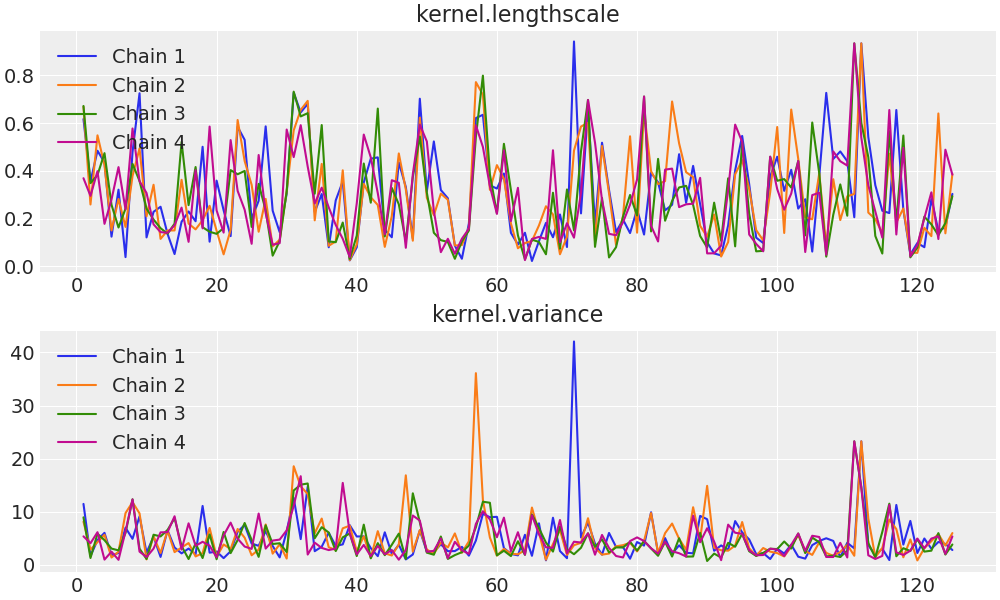
\includegraphics[width=0.5\textwidth]{src/traceplots.png}
    \caption{Trace plots of the Markov chains.}
    \label{fig:mcmc}
\end{figure}

\begin{table}[H]
\centering
\resizebox{\textwidth}{!}{\begin{tabular}{lrrrrrrrrr}
\toprule
{} &   mean &     sd &  hdi\_2.5\% &  hdi\_97.5\% &  mcse\_mean &  mcse\_sd &  ess\_bulk &  ess\_tail &  r\_hat \\
\midrule
kernel.lengthscale &  0.294 &  0.191 &     0.022 &      0.657 &      0.017 &    0.012 &     111.0 &     247.0 &   1.01 \\
kernel.variance    &  4.792 &  4.144 &     0.743 &     11.903 &      0.314 &    0.222 &     206.0 &     135.0 &   1.01 \\
\bottomrule
\end{tabular}}
\caption[]{Diagnostics of MCMC samples generated by NUTS.}
\label{tab:mcmc}
\end{table}

Based on the diagnostics in \autoref{appendix2}, we obtain our final 500 samples from $p(\bm{\theta}|\mathcal{D})$ using four chains, but this time with a warm-up period of 10 for each chain. Diagnostics for our final sample is given in \autoref{fig:mcmc} and \autoref{tab:mcmc} A scatter plot of the samples on log-log-scale is given \autoref{fig:loglog} and a plot of the posterior predictive is given in \autoref{fig:postpred}.

\begin{figure}[H]
        \centering
        \begin{subfigure}[b]{0.475\textwidth}
            \centering
            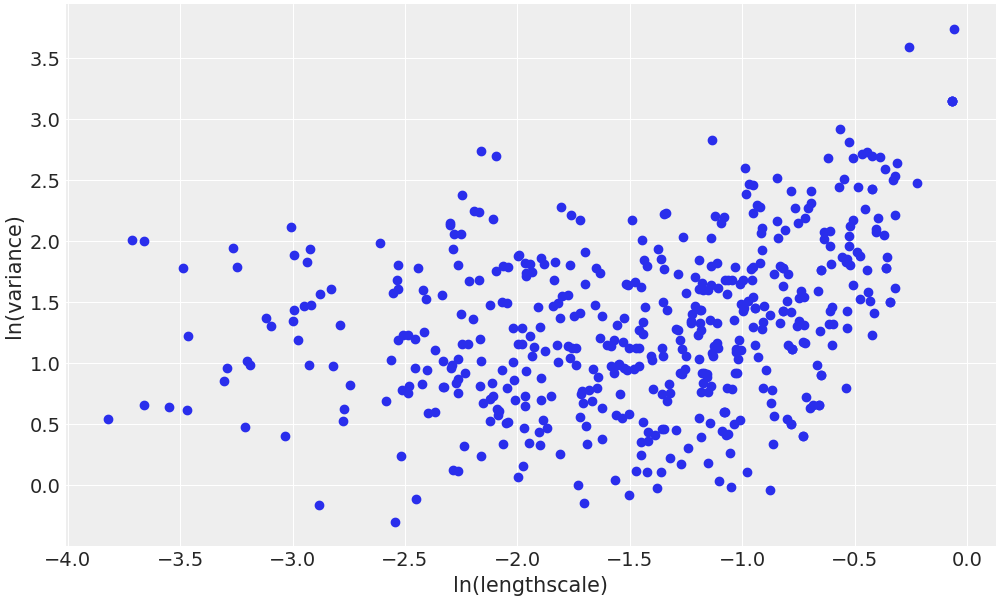
\includegraphics[width=\textwidth]{src/loglogplot.png}
            \caption{}
            \label{fig:loglog}
        \end{subfigure}
        \hfill
        \begin{subfigure}[b]{0.475\textwidth}  
            \centering 
            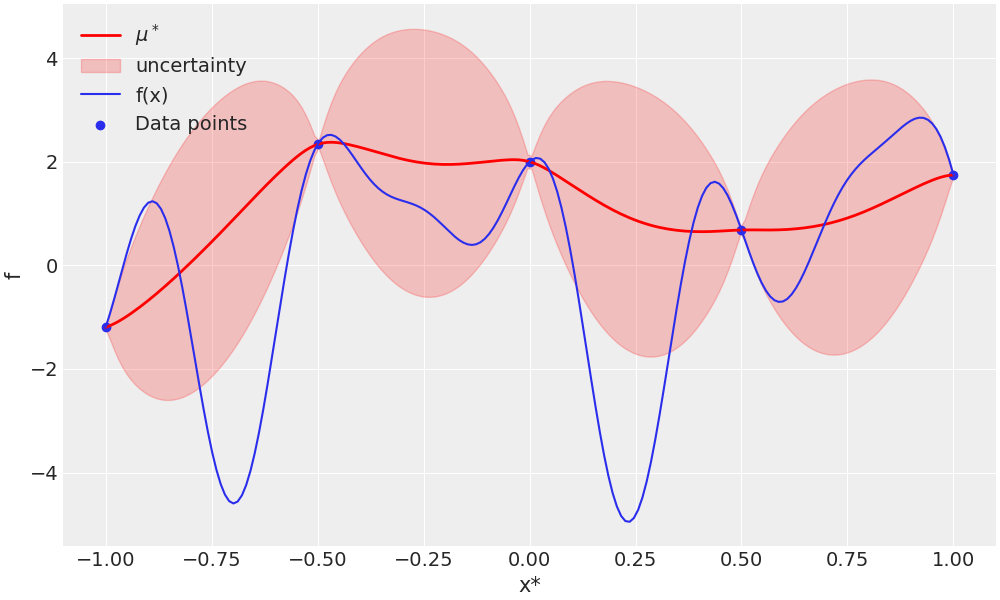
\includegraphics[width=\textwidth]{src/posteriorpred.png}
            \caption{}
            \label{fig:postpred}
        \end{subfigure}
        \caption[]
        {(a) Scatter plot on log-log scale of $N=500$ samples from $p(\bm{\theta}|\mathcal{D})$, (b) $p(f^*|x^*,\mathcal{D})$ for $x^*\in[-1, 1]$.} 
        \label{fig:targetsmulti}
    \end{figure}


\subsection*{B.2 – Bayesian Optimization}

\subsubsection*{Deliverable 1 \& 2}
We consider algorithm 1 in a setting with $T=50$ iterations and $n=20$ repetitions. To ensure convergence of the MCMC chain to its stationary distribution, we deem that a warm-up period of 10 samples is sufficient. We show the sampled $f^*$ at iterations $k=$0, 5, 10 in \autoref{fig:algorithm1} and \autoref{fig:performance1}, and \autoref{tab:avgiter} provide a summary of the above setting.

\begin{figure}[H]
    \centering
    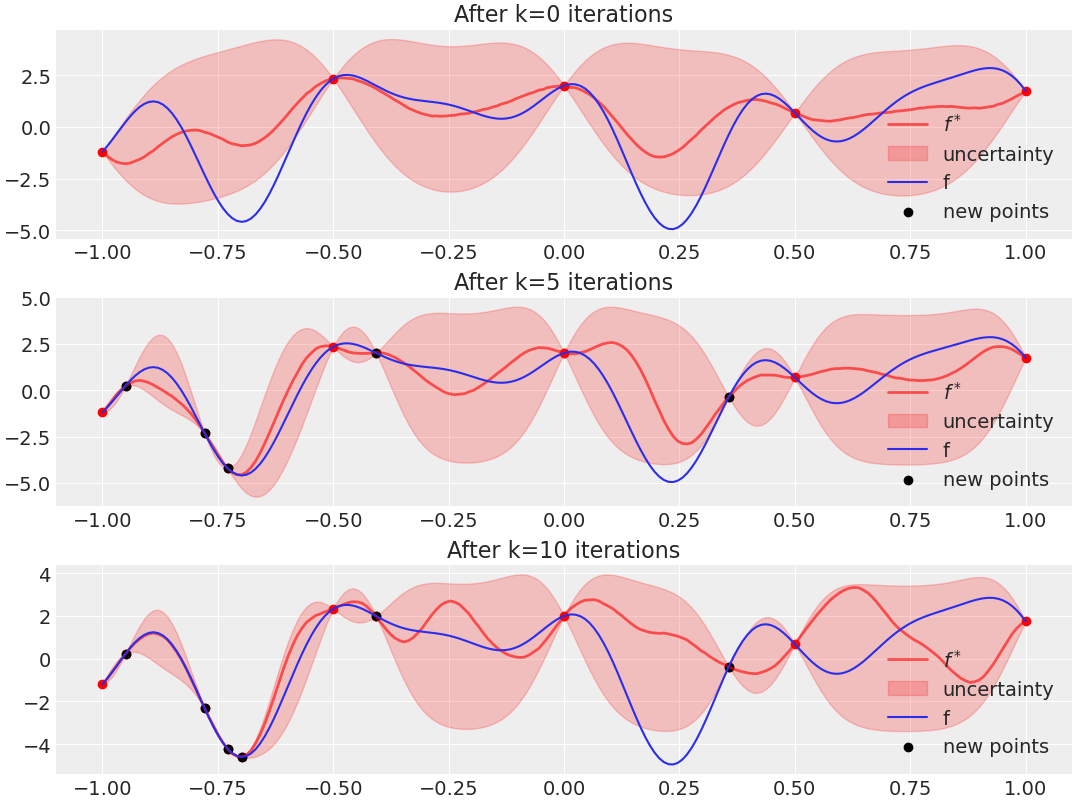
\includegraphics[width=0.475\textwidth]{src/algorithm1plot.png}
    \caption{Sampled $f^*$, $f$, and  $p(f^*|x^*,\mathcal{D}, \bm{\theta}^{(k)})$ at $k=$0,5,10 iterations.}
    \label{fig:algorithm1}
\end{figure}
By inspection of \autoref{fig:performance1} we note that algorithm 1 (denoted alg\_1\_RBF) did not manage to find global optimum in 7 out of 50 repetitions, which is indicated by values of zero. In particular, the decision rule implies that the algorithm in some repetitions becomes overconfident in regions with local optima. Thus, there is a very low probability that values of the sampled $f^*$ in the region of the global optimum will lie below the value of the sampled $f^*$ in the region of the local optimum, and hence a low probability that the algorithm will explore the region of the global optimum. This is evident from \autoref{fig:algorithm1}, where the probability that the sampled value of $f^*$ in the region of the global optimum attains a value that lies below the sampled value of $f^*$ in the region of the local optimum is less than 0.025\footnote{This can be deduced by noting that $f^*$ in the region of the global optimum must attain a value that lies more than two standard deviations away from the mean. Values two standard deviations above the mean are not relevant, hence 0.025.}.

\subsubsection*{Deliverable 3}
One immediate extension to ensure that the algorithm eventually will find the global minimum is to not allow for repeated decisions in terms of the added point, $(x_p^*, f(x_p^*))$. In this way, the algorithm is forced to explore alternative optima by considering the optimal point among the set of points, in which the previous sampled points are not included. Since $f(x)$ is assumed to be noiseless, no information is gained by resampling the same point. We denote this algorithm 1.1. Another alternative is to incorporate the information contained in $p(f^*|x^*,\mathcal{D},\bm{\theta}^{(i)})$ directly into the decision rule. One way to do so is the GP-LCB algorithm proposed by \cite{Srinivas_2012}, where the decision rule is given by:
\begin{equation}
    x_p^* = \argmin_i \left\{ \mu_{\bm{\theta}}^*(x_i^*) - \sqrt{\beta}_k \sigma_{\bm{\theta}}^*(x_i^*)\right\}, \qquad \beta_k = \phi\cdot\ln(k)
\end{equation}
Where $\phi$ is a confidence parameter. GP-LCB follows the 'optimism in face of uncertainty principle', in which we choose optimistic candidate points taking into account the variance of the GP. Note, however, that the success of the algorithm crucially relies on $\beta_k$ being increasing as a function of $\ln(k)$. Otherwise, GP-LCB will run into the same pitfalls as algorithm 1. Likewise, if $\phi$ is set too low, GP-LCB will become overconfident and get stuck in local optima for many iterations\footnote{On the other hand, it should also not be set too high so that the algorithm is too exploratory. In either case, it will converge to the optimum eventually as long as $\beta_k$ is increasing as a function of $\ln(k)$.}. Intuitively, when $\beta_k$ increases as a function of $\ln(k)$, $\sqrt{\beta_k}\sigma_{\bm{\theta}}^*(x^*)$ evaluated in regions with high uncertainty will eventually become larger than the $\sqrt{\beta_k}\sigma_{\bm{\theta}}^*(x^*)$ evaluated in regions with low uncertainty, since the magnitude of $\sigma_{\bm{\theta}}^*(x^*)$ will be larger in regions with higher uncertainty. In this way it is ensured that GP-LCB will never become overconfident in local optima regions, as it will eventually explore regions with higher uncertainties.\\
Another way to make the algorithms more exploratory can be induced by choosing a kernel with higher uncertainty estimates either through the kernel type itself or through the prior for the hyperparameters. The exploratory nature of our sampled $f^*$ from $p(f^*|x^*,\mathcal{D}, \bm{\theta}^{(k)})$ is primarily determined by the sampled $\bm{\theta}^{(k)}$ from $p(\bm{\theta}|\mathcal{D})$. That is, if we compare the behaviour of $f^*$ using a Matérn 3/2 kernel, it will explore much of the same space as with a RBF kernel for most of the sampled values from $p(\bm{\theta}|\mathcal{D})$ (which is also suggested by the results in \autoref{fig:performanceplots}). Thus, we induce more exploration by introducing a new prior, $\sigma_\mathit{s}^2\sim\text{LogNormal}(1.7, 0.3)$, and use a Matérn 3/2 kernel as a robustness check. \autoref{fig:performanceplots} and \autoref{tab:avgiter} provide a summary of the experiment with $\phi=2$. Evidently, a prior favoring larger values of $\sigma_\mathit{s}^2$ can by itself alleviate the issue of algorithm 1 getting stuck in local optima.

\begin{figure}[H]
        \centering
        \begin{subfigure}[b]{0.475\textwidth}
            \centering
            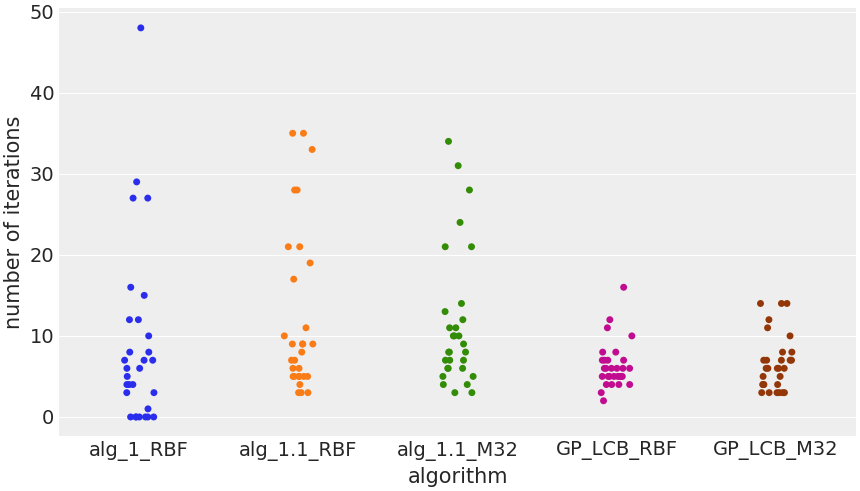
\includegraphics[width=\textwidth]{src/performanceplotorignalprior.png}
            \caption{}
            \label{fig:performance1}
        \end{subfigure}
        \hfill
        \begin{subfigure}[b]{0.475\textwidth}  
            \centering 
            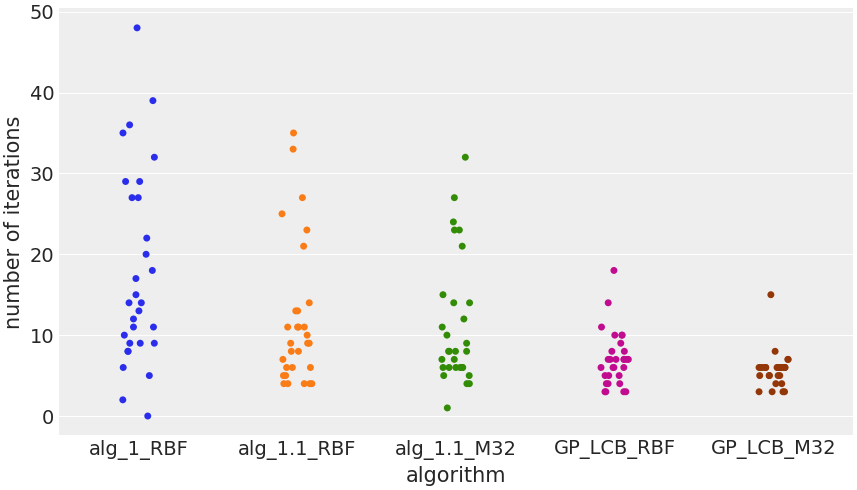
\includegraphics[width=\textwidth]{src/performanceplotsnewprior.png}
            \caption{}
            \label{fig:performance2}
        \end{subfigure}
        \caption[]
        {Number of iterations until global minimum is found. 0 iterations indicate that the that the global is never found. (a) With $\sigma_\mathit{s}^2\sim\text{LogNormal}(0, 2)$ (b) With $\sigma_\mathit{s}^2\sim\text{LogNormal}(1.7, 0.3)$.} 
        \label{fig:performanceplots}
\end{figure}
    
\begin{table}[H]
\centering
\resizebox{12cm}{!}{\begin{tabular}{llllllr}
\toprule
  &  alg\_1\_RBF & alg\_1.1\_RBF & alg\_1.1\_M32 & GP\_LCB\_RBF &  GP\_LCB\_M32 \\
\midrule
 $\sigma_\mathit{s}\sim\text{LogNormal}(0, 2)$ & 20.63 &  12.36  &   11.53 &   6.33 &  6.67 \\
 $\sigma_\mathit{s}\sim\text{LogNormal}(1.7, 0.3)$ & 19.50 &  11.87  &   11.20 &   7.00 &  5.73 \\
\bottomrule
\end{tabular}}
\caption[]{Average number of iterations until global minimum is found. Note that alg\_1\_RBF counts 50 iterations in the average when the global minimum is not found.}
\label{tab:avgiter}
\end{table}

\iffalse

\newpage
\textbf{I praksis giver Matern kernel ikke meget mere uncertainty end RBF kernel (på trods af Oswins script indikerer det). Det afhænger i højere grad af sampled lengthscale og sampled variance. Derfor er følgende lidt forkert. }For instance, choosing $\kappa=1$ will produce good results with a Matérn 5/2 kernel, but poor results with a RBF kernel. On the other hand, choosing $\kappa=4$ will produce opposite results, as the Matérn 5/2 kernel induces too much exploration. Note however, that since we found that algorithm 1 wasn't exploratory enough, a Matérn 5/2 kernel by itself can improve algorithm 1. \textbf{I og med der ikke er nogen $\phi$-parameter i algorithm 1, så kan Matern kernel 5/2 i sig selv hjælpe betydeligt på algoritme 1, da den inducerer højere varians, og dermed mere exploratory!!}\\
Summary statistics for our preferred choice of GP-LCB initialization using the RBF kernel is given in table ?.\\
table/figure here\
\fi

\iffalse
Since we are investigating the predictive posterior we need to only sample a single from the posterior of the parameters $p(\bm{\theta} \vert \mathcal{D})$, however, this does not imply we can sample a single point in each iteration, get a new data point and $(x^*_p, y^*_p)$, and run a single iteration of the Markov chain to get a new sample of the posterior. This is due to two reasons. First, the samples from the posterior $p(\bm{\theta} \vert \mathcal{D})$ needs to be \textit{i.i.d}, to be representative samples when sampling the predictive posterior. However, Markov chains does in practice show a degree of auto-correlation between samples, so the chain needs to run for some time between two draws to ensure, that the samples from the posterior in fact are  \textit{i.i.d.} Second point is, that $f^*$ do need to be sampled from the posterior of $f^* \sim p(f^* \vert X, \mathcal{D})$. We need to take into account, that the dataset $\mathcal{D}$ is updated, that is $\mathcal{D} \leftarrow \mathcal{D} \cup \{(x^*_p, y^*_p)\}$, why we need to run the Markov chain to update the posterior once more.

\textbf{Deliverable 1:}

\textbf{Deliverable 2:}

\textbf{Deliverable 3:} As alluded to in the question, there are 3 obvious approaches to improve the algorithm. 1) kernel SKRIV. 2) prior SKRIV. 3) We can consider, if there are more efficient ways to search for points. Since the setup in this assignment requires us to consider 200 evenly spaced index points in the interval $[-1, 1]$, two obvious considerations can be made. First, and the most simple way to improve the algorithm is to remove already investigated points. Since we have fixed the variance of $y$ to be very small (non existent), then, when we have evaluated a point in $f(\cdot) $ a single time, we have ground truth of the specific point. In other words, if we again would redraw that point, we cannot gain any additional information. Second thing to consider is, how we trade off exploitation and exploration. We can very easily end up in a region of the optimization problem, where we have low expected outcome, and keep exploiting this region. We therefore need to employ an algorithm that let us efficiently search over not just a local maximum put the entire search space. For this we choose the online learning approach called Gaussian Process Lower Confidence Bound (CITÉR SRINIVASAN 2012). Formally this implies:

\begin{equation}
    x_i^* = argmin \left\{ \mu(x_i) - \sqrt{\beta}_t \sigma(x_i)\right\}, \qquad \beta_t = g(\ln(t), \kappa)
\end{equation}

where $\kappa$ is a set of hyper parameters.

\fi

\newpage

\bibliography{src/references}

\newpage

\begin{appendices}

\section{Visualization of generated images}\label{appendiximages}


\section{Posterior predictive distribution}\label{appendix1}
The posterior predictive distribution is given by:
\begin{align}
    p(f^*|x^*,\mathcal{D}) &= \int_{\Omega_{\bm{\theta}}}p(f^*,{\bm{\theta}}|x^*,\mathcal{D})d{\bm{\theta}}\\
    &=\int_{\Omega_{\bm{\theta}}}p(f^*|x^*,\mathcal{D},{\bm{\theta}})p({\bm{\theta}}|\mathcal{D})d{\bm{\theta}}\\
    &=\mathbb{E}_{{\bm{\theta}}\sim p({\bm{\theta}}|\mathcal{D})}\left[p(f^*|x^*,\mathcal{D},{\bm{\theta}})\right]\\
    &\approx N^{-1}\sum_{i=1}^N p(f^*|x^*,\mathcal{D}, {\bm{\theta}}^{(i)})
\end{align}
Where M denotes the number of samples, and:
\begin{equation}
    p(f^*|x^*,\mathcal{D}, {\bm{\theta}}^{(i)}) \sim \mathcal{N}\left(\mu_i^*, \, \, (\sigma_i^2)^*\right)
\end{equation}
Where: 
\begin{align*}
    &\mu_i^*=k_{{\bm{\theta}}^{(i)}}(S,x^*)^Tk_{{\bm{\theta}}^{(i)}}^{-1}y\\
    &(\sigma_i^2)^*=k_{{\bm{\theta}}^{(i)}}(x^*,x^*)-k_{{\bm{\theta}}^{(i)}}(S,x^*)^TK(S)^{-1}k_{{\bm{\theta}}^{(i)}}(S,x^*)
\end{align*}

\section{MCMC diagnostics for assessing mixing and required warm-up period}\label{appendix2}

\begin{figure}[H]
    \centering
    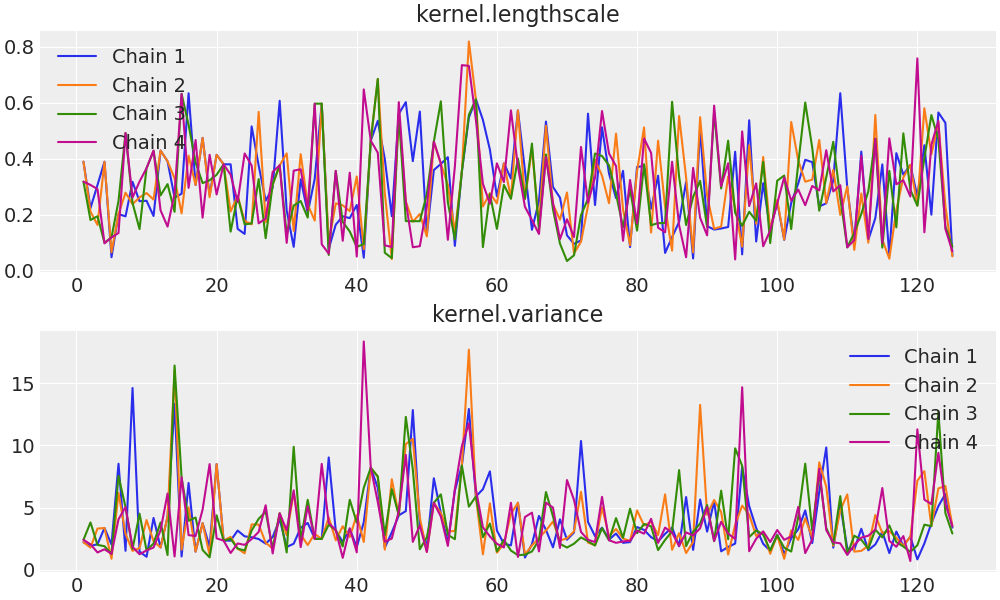
\includegraphics[width=0.5\textwidth]{src/traceplotsdiagnostics.png}
    \caption{Trace plots of the Markov chains with no warm-up period.}
    \label{fig:mcmcdiag}
\end{figure}

\begin{table}[H]
\centering
\resizebox{\textwidth}{!}{\begin{tabular}{lrrrrrrrrr}
\toprule
{} &   mean &     sd &  hdi\_2.5\% &  hdi\_97.5\% &  mcse\_mean &  mcse\_sd &  ess\_bulk &  ess\_tail &  r\_hat \\
\midrule
kernel.lengthscale &  0.296 &  0.157 &     0.043 &      0.596 &      0.012 &    0.009 &     167.0 &     169.0 &   1.04 \\
kernel.variance    &  3.820 &  2.698 &     0.706 &      8.632 &      0.232 &    0.165 &     154.0 &     228.0 &   1.03 \\
\bottomrule
\end{tabular}}
\caption[]{Diagnostics of MCMC samples generated by NUTS with no warm-up period.}
\label{tab:mcmcdiag}
\end{table}

\end{appendices}



\end{document}
